\documentclass[11pt]{article}
\usepackage{amsfonts}
\usepackage{amsmath}
\usepackage{cancel}
\usepackage{mathtools}
\usepackage{graphicx}
\setlength{\pdfpagewidth}{8.5in}
\setlength{\pdfpageheight}{11in}
\textwidth 6.5in
\textheight 9in
\headheight 0.0in
\topmargin -.5in
\oddsidemargin 0.0in
\evensidemargin 0.0in

\title{\bf CS 181 - Homework 1}
\date{\today}
\author{Lexi Ross \& Ye Zhao}
\begin{document}
\maketitle
\section{Decision Tree \& ID3}

\section{ID3 with Pruning}

\section{Boosting}

\subsection{Information gain criterion using weights}
In order to take into account weights when calculating the information gain of a given attribute, we use the following formula to calculate the entropy of the labels:
$$H(\text{labels})=\sum_{c=1}^{C}\frac{W_c}{W}\log_2\frac{W}{W_c}$$
Where $$W_c = \sum_{n=1}^{N}I(y_n=c)w_n$$ and $$W=\sum_{n=1}^{N}w_n$$
We chose this information gain criterion because it came from the lecture slides, and it is a natural extension of the formula for unweighted label entropy. Instead of looking at the ratio of the number of examples possessing a given label to the total number of examples, we sum the weights of these examples. In other words, unweighted entropy is a specific case of weighted entropy, where the weight of each example is 1.

\subsection{Effect of maximum depth of weak learner}
\begin{center}
\begin{tabular}{c c l c}
Max. depth & Boosting rounds & Dataset & Test performance \\ \hline
1 & 10 & non-noisy & 0.89 \\ \hline
1 & 10 & noisy & 0.82 \\ \hline
1 & 30 & non-noisy & 0.91 \\ \hline
1 & 30 & noisy & 0.84 \\ \hline \hline
2 & 10 & non-noisy & 0.87 \\ \hline
2 & 10 & noisy & 0.81 \\ \hline
2 & 30 & non-noisy & 0.87 \\ \hline
2 & 30 & noisy & 0.79 \\ \hline
\end{tabular}
\end{center}
Interestingly, increasing the max depth of the weak learner worsens the testing accuracy when controlling for both boosting rounds and noise level. The gap is significantly larger for 30 rounds of boosting than for 10 rounds, suggesting that overfitting is taking place, increasing in magnitude with each round of AdaBoost. It appears that a max depth of 1 (i.e. a decision stump) is the optimal weak learner to use. Something else interesting happens with a max depth of two: in the non-noisy dataset, a training error of zero is achieved within the first ten rounds of boosting (in fact, it is achieved in the very first round). Because we exit from AdaBoost once we find a tree that perfectly fits the training data, we subject ourselves to the dangers of overfitting***. Indeed, the largest discrepancy between the training accuracy and test accuracy occurs in this case. In addition, for cases like these, adding rounds of AdaBoost does not improve test accuracy.

\subsection{Cross-validated test performance over different numbers of boosting rounds}
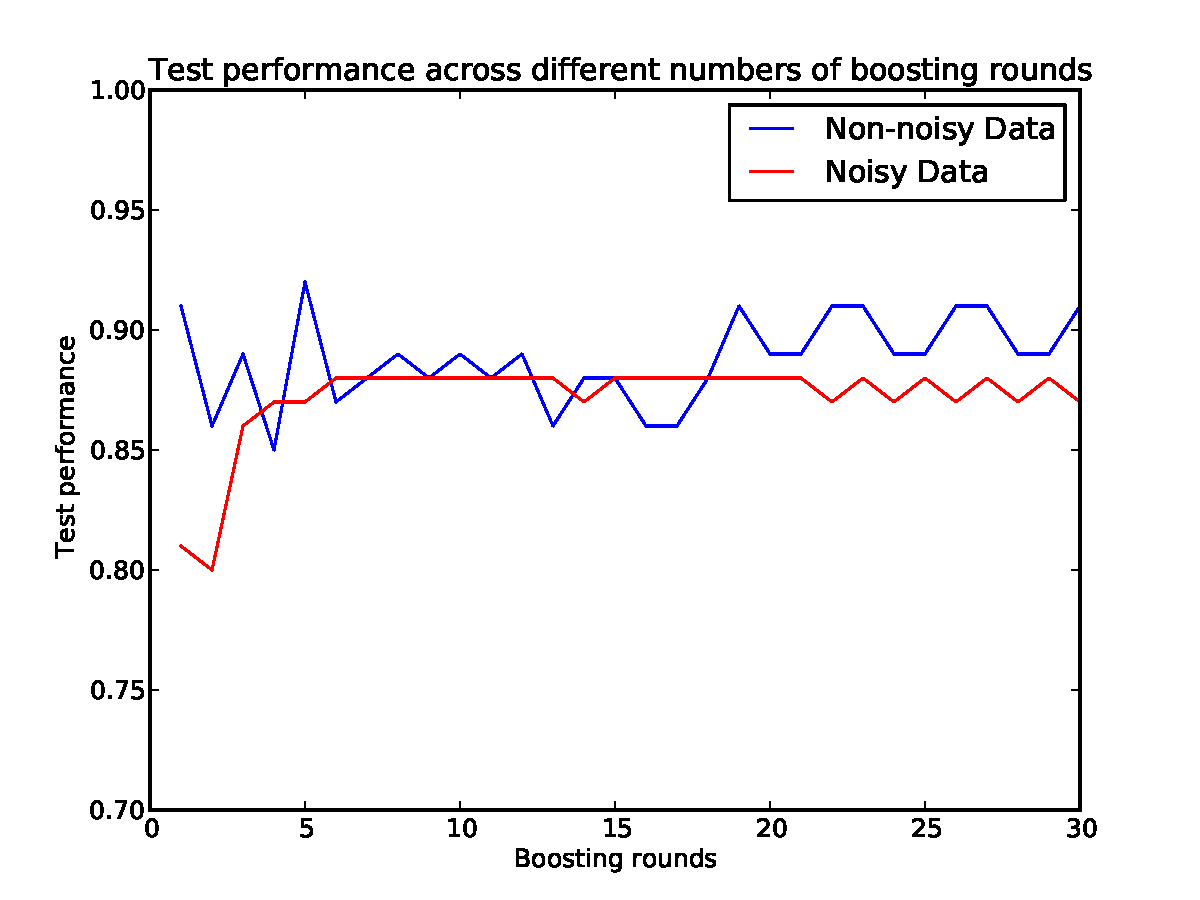
\includegraphics[scale=0.8]{graph3b}
For both datasets, test performance fluctuates greatly during the first 10-12 rounds and then improves slightly before remaining at a fairly constant value for the last 10 rounds. As we would expect, the noisy dataset sees more variation between rounds, including in later rounds; this is indicative of invalid data points being classified incorrectly by accurate weak learners and subsequently gaining a lot of weight. For this reason, noise is particularly bad for boosting. We were initially surprised that performance did not increase monotonically with each round, as it should in theory, but our implementation of AdaBoost (and the weighting computations in dtree.py) do not guarantee that the redistribution of weights will lead to a strictly more accurate learner with a higher tree weight, particularly when it comes to test data. The accuracy did improve overall from 1 to 30 rounds (for both datasets), which was expected: more rounds of boosting should lead to better results, because boosting is particularly resistant to over fitting.

\subsection{Boosting vs. ID3 with and without pruning}
Without pruning, ID3 gives a cross-validated test performance of 0.87 on the non-noisy dataset. Using optimal parameters (30 rounds, max depth of 1), boosting can significantly improve that performance -- to 0.91. However, when max depth was increased to 2, boosting merely matched the raw ID3 performance. 

\subsection{Test vs. training performance over different numbers of boosting rounds}
When testing the non-noisy dataset with weak learners of max depth 1, the training accuracy starts off extremely high (0.953333) and increases slightly every several rounds, reaching a steady state at 9 rounds with 0.957778. The testing performance, on the other hand, starts at 0.88 and increases every several rounds at a faster rate than the training performance (although test performance is always worse than training performance). Interestingly, test performance reaches and maintains its maximum at 12 rounds, 3 rounds later than the training performance stopped increasing. This speaks to the remarkable property of AdaBoost that allows it to improve test performance even after training performance has maxed out (again, its resistance to over fitting).

\section{Tree Analysis}
The following tree was generating using AdaBoost, with a maximum depth of 1 on weak learners and 21 rounds of boosting. We examined the resulting decision trees throughout boosting, and noticed that this dataset was producing particularly robust decision trees, such that each round of boosting changed very little about the structure of the tree, and error was very low from the beginning. Therefore, we extracted the first tree from the set of hypotheses and ran it through our cross validation function (such that the same tree was tested on all ten folds). We found a test performance of 0.95.\\
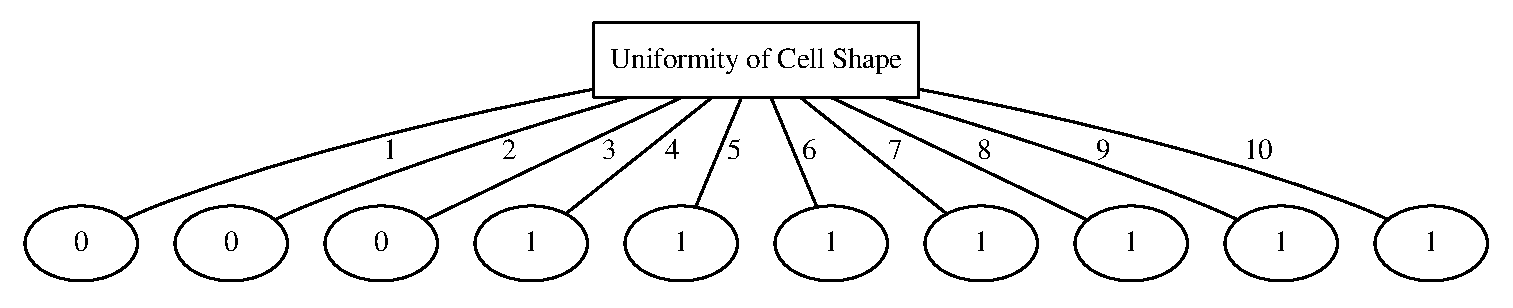
\includegraphics[scale=0.75]{tree_pt4_alternate}
According this tree, the most important attribute when determining benign/malignant decisions is the uniformity of cell shape in the tumor. Lower values of uniformity (less than or equal to 3) lead to 0 labels (indicating a benign tumor), while higher values tend to produce 1 labels (malignant). \\

Because this decision stump encapsulates so little information about the original dataset, we wondered whether a deeper tree would lead to more accurate results. While we were able to reach a test performance of 0.99, the tree itself because exponentially more complex (see below), so we decided to stick with the decision stump. For this deeper tree, however, we can branch on clump thickness and single epithelial cell size. \\
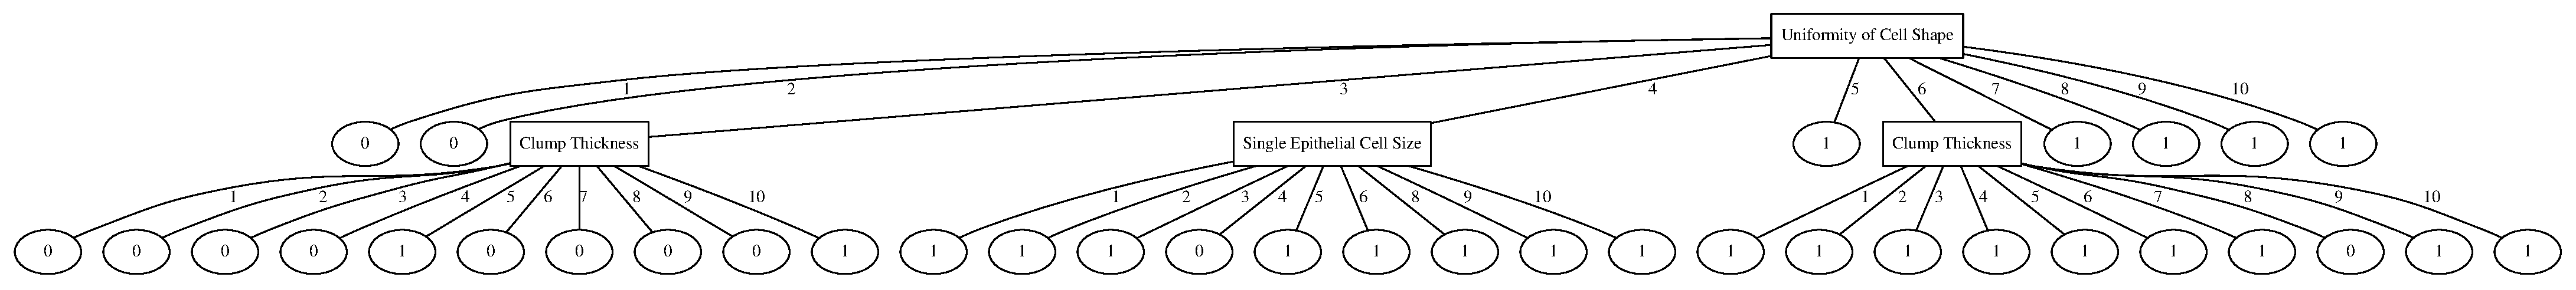
\includegraphics[scale=0.25]{tree_pt4}

\end{document}